\documentclass[12pt,a4paper]{article}
\usepackage{amsmath,amscd,amsbsy,amssymb,latexsym,url,bm,amsthm}
\usepackage{epsfig,graphicx,subfigure}
\usepackage{enumitem,balance}
\usepackage{wrapfig}
\usepackage{mathrsfs, euscript}
\usepackage[usenames]{xcolor}
\usepackage{hyperref}
\usepackage[vlined,ruled,commentsnumbered,linesnumbered]{algorithm2e}
\usepackage{float}
\usepackage{array}
\usepackage{diagbox}
\usepackage{color}
\usepackage{indentfirst}
\usepackage{fancyhdr}
\usepackage{gensymb}
\usepackage{geometry}
\usepackage{setspace}
\usepackage{aurical}
\usepackage{times}
\usepackage{caption}
\usepackage{fontspec}
\usepackage{booktabs}
\setmainfont{Times New Roman}

\newtheorem{theorem}{Theorem}[section]
\newtheorem{lemma}[theorem]{Lemma}
\newtheorem{proposition}[theorem]{Proposition}
\newtheorem{corollary}[theorem]{Corollary}
\newtheorem{exercise}{Exercise}[section]
\newtheorem*{solution}{Solution}
\theoremstyle{definition}

\newcommand{\postscript}[2]
 {\setlength{\epsfxsize}{#2\hsize}
  \centerline{\epsfbox{#1}}}
\renewcommand{\baselinestretch}{1.0}

\setlength{\oddsidemargin}{-0.365in}
\setlength{\evensidemargin}{-0.365in}
\setlength{\topmargin}{-0.3in}
\setlength{\headheight}{0in}
\setlength{\headsep}{0in}
\setlength{\textheight}{10.1in}
\setlength{\textwidth}{7in}
\makeatletter \renewenvironment{proof}[1][Proof] {\par\pushQED{\qed}\normalfont\topsep6\p@\@plus6\p@\relax\trivlist\item[\hskip\labelsep\bfseries#1\@addpunct{.}]\ignorespaces}{\popQED\endtrivlist\@endpefalse} \makeatother
\makeatletter
\renewenvironment{solution}[1][Solution] {\par\pushQED{\qed}\normalfont\topsep6\p@\@plus6\p@\relax\trivlist\item[\hskip\labelsep\bfseries#1\@addpunct{.}]\ignorespaces}{\popQED\endtrivlist\@endpefalse} \makeatother

\begin{document}
\noindent
%==========================================================
\noindent\framebox[\linewidth]{\shortstack[c]{
\Large{\textbf{Report on Homework 2}}\vspace{1mm}\\ 
CS420, Machine Learning, Shikui Tu, Summer 2018 \vspace{1mm} \\
Zelin Ye 515030910468}}

\section{PCA algorithm}

\subsection{Original PCA}
When it comes to principal component, the most common used approach is principal component analysis (PCA) algorithm. Thus, I can use the original PCA algorithm to extract the first principal component of the dataset. The computational details can refer to Alg. \ref{alg:pca_1}.

\vspace{0.01\linewidth}
\begin{algorithm}[H]
	\SetKwInOut{Input}{Input}
	\SetKwInOut{Output}{Output}
	\caption{Original PCA}
	\label{alg:pca_1}
	\vspace{0.25\baselineskip}
	
	\Input{The dataset $X$, a $n \times N$ matrix}
	\Output{The first principal component $w$}
	%Rearrange the dataset $X$ by
	%\begin{equation*}
	%	\centering
	%	X \leftarrow X^T,
	%\end{equation*}
	%so that each line denotes one data point;
	
	Conduct normalization for $X$, and make sure the mean of $X$ is 0;
	
	Find the covariance matrix of $X$, denoted by $C$:
	\begin{equation*}
		\centering
		C \leftarrow XX^{T};
	\end{equation*}
	
	Calculate the eigenvalues $\lambda$ and eigenvectors $V$ of $X$;
	
	Choose the maximal eigenvalue $\lambda_{m}$ and corresponding eigenvector $v_{m}$;
	
	Calculate the first principal component:
	\begin{equation*}
		\centering
		w \leftarrow v_{m}^{T}X;
	\end{equation*}
	
	\Return $w$;
\end{algorithm}
\vspace{0.01\linewidth}

The above algorithm (PCA) is a classical and commonly used method to solve principal components, which has the following characteristics.

\vspace{-0.012\linewidth}
\paragraph{Pros:}
\begin{enumerate}
	\item PCA has simple logic and is easy to implement;
	
	\item The orthogonality among principal components chosen by PCA can eliminate the interaction between original data components;
	
	\item PCA belongs to unsupervised learning, and it is not restricted by sample labels.
\end{enumerate}

\vspace{-0.03\linewidth}
\paragraph{Cons:}
\begin{enumerate}
	\item PCA treats all samples, namely the collection of eigenvectors, as a whole and neglects the category attributes. Nevertheless, the projection direction it neglects might contain some important separability information;
	
	\item PCA would be time-consuming when encountering large amount of data;
	
	\item The actual meanings of principal components extracted by PCA are a little bit ad-hoc and hard to explain.
\end{enumerate}

\subsection{SVD}
In fact, I can also extract principle components via SVD (Singular Value Decomposition), which is a way to decompose a matrix as the following equation. 

\begin{equation*}
	\centering
	X_{m \times n} = U_{m \times m} \Sigma_{m \times n} V^T_{n \times n},
\end{equation*}
where $\Sigma$ is a diagonal matrix, and the values on the diagonal are called the singular values. The vectors in $U$ and $V$ are orthogonal.

In most cases, the sum of singular values of the first 10\% or even 1\% accounts for more than 99\% of the sum of all singular values. Therefore, I can obtain first principle components through the biggest singular value. Corresponding details can refer to Alg. \ref{alg:svd}.

\vspace{0.01\linewidth}
\begin{algorithm}[H]
	\SetKwInOut{Input}{Input}
	\SetKwInOut{Output}{Output}
	\caption{SVD}
	\label{alg:svd}
	\vspace{0.25\baselineskip}
	
	\Input{The dataset $X$, a $n \times N$ matrix}
	\Output{The first principal component $w$}
	
	Conduct normalization for $X$, and make sure the mean of $X$ is 0;
	
	Carry out SVD for $X$:
	\begin{equation*}
		\centering
		X \leftarrow U \Sigma V^T;
	\end{equation*}
	
	Multiply the transposition of matrix $U$ on both sides of the above formula:
	\begin{equation*}
		\centering
		U^TX \leftarrow \Sigma V^T;
	\end{equation*}
	
	Then the compression of original data is $\Sigma V^T$, denoted by $X^{'}$;
	
	Assign the first row of $X^{'}$ to $w$;
	
	\Return $w$;
\end{algorithm}
\vspace{0.01\linewidth}

Actually, PCA is a wrapper of SVD, SVD is usually used as a implementation of PCA (e.g. sklearn). In addition to most of the characteristics of PCA, SVD has the following ones:

\vspace{-0.012\linewidth}
\paragraph{Pros:}
\begin{enumerate}
	\item SVD could handle matrices that are not square matrices, while the eigenvalue decomposition in PCA is only applicable to the square matrices;
	
	\item Different from PCA, there is no need for SVD to calculate $XX^T$, where some small values in $X$ might be lost in squares;
	
	\item SVD can extract the principle components of two directions. For instance, if I multiply $V$ on both sides of $X=U \Sigma V^T$, I will implement the compression on samples, namely merge some similar samples or eliminate those inconsequential ones. Whereas, PCA cannot achieve this.
\end{enumerate}

\vspace{-0.03\linewidth}
\paragraph{Cons:}
\begin{enumerate}
	\item The complexity of calculating the singular values is $O(N^3)$, which is not suitable for large scale samples. Parallel computing can solve this problem a little bit;
	
	\item The compression results of SVD are lack of interpretability.
\end{enumerate}

\subsection{KPCA}
The original PCA and SVD might have good performance when handling linear data, but it would encounter difficulties under non-linear data. In non-linear cases, a variant of PCA called KPCA (kernel principal components analysis) shows its strength.

The innovation of KPCA is that it introduces a non-linear mapping function $\phi(x)$, mapping the data from original space to high-dimensional space. Besides, the deduction of KPCA takes advantage of the theorem that \textit{each vector in the space could be expressed linearly by all the samples in the space}. The details of KPCA can refer to Alg. \ref{alg:pca_2}.

\vspace{0.01\linewidth}
\begin{algorithm}[H]
	\SetKwInOut{Input}{Input}
	\SetKwInOut{Output}{Output}
	\caption{KPCA}
	\label{alg:pca_2}
	\vspace{0.25\baselineskip}
	
	\Input{The dataset $X$, a $n \times N$ matrix; kernel function $\phi(x)$}
	\Output{The first principal component $w$}	
	Conduct normalization for $X$, and make sure the mean of $X$ is 0;
	
	Calculate kernel matrix $K$:
	\begin{equation*}
		\centering
		K \leftarrow X^{T}X,
	\end{equation*}
	where $X=[\phi(x_1),...,\phi(x_N)]$;
	
	Find the covariance matrix of $X$, denoted by $C$:
	\begin{equation*}
		\centering
		C \leftarrow XX^{T};
	\end{equation*}
	
	Calculate the eigenvalues $\lambda$ and eigenvectors $U$ of $K$;
	
	Choose the maximal eigenvalue $\lambda_{m}$ and calculate corresponding eigenvector $u_{m}$;
	
	Calculate the corresponding eigenvectors $v_m$ of covariance matrix $C$ by $u_m$:
	\begin{align*}
		\centering
		v_m &\leftarrow \dfrac{1}{\|X^Tu_m\|}X^Tu_m \\
		&= \dfrac{1}{\sqrt{u_m^TXX^Tu_m}}X^Tu_m \\
		&= \dfrac{1}{\sqrt{u_m^T(\lambda_m u_m)}}X^Tu_m \\
		&= \dfrac{1}{\sqrt{\lambda_m}}X^Tu_m;
	\end{align*}
		
	Calculate the first principal component:
	\begin{equation*}
		\centering
		w \leftarrow v_{m}^{T}X;
	\end{equation*}
	
	\Return $w$;
\end{algorithm}
\vspace{0.01\linewidth}

KPCA is a ingenious extension of PCA, and is also widely used (e.g. dimension reduction, clustering). The pros and cons of KPCA are as follows.

\vspace{-0.012\linewidth}
\paragraph{Pros:}
\begin{enumerate}
	\item Basically, KPCA owns almost all of the advantages of PCA;

	\item KPCA has a stronger universality, which could find out the non-linear information contained in dataset;
	
	\item KPCA uses simple kernel functions (e.g. polynomial kernel function) to realize complex non-linear transform;
\end{enumerate}

\vspace{-0.03\linewidth}
\paragraph{Cons:}
\begin{enumerate}
	\item The logic and implementation of KPCA is a little bit complicated;
	
	\item The dimension of kernel matrix $K$ is $N \times N$ ($N$ is the number of samples). It might take quantities of time to process $K$ when handling large scale of samples;
	
	\item Different choices of kernel functions and parameters would affect the result to a certain extent, which makes this algorithm more tricky.
	
	\item Same as PCA and SVD, the actual meanings of principal components extracted by KPCA are also inexplicable.
\end{enumerate}

\section{Factor Analysis (FA)}

\vspace{-0.03\linewidth}
\begin{large}
\begin{align*}
	\centering	
	p(y|x) &= \dfrac{p(x|y)p(y)}{p(x)} \\
	&= \dfrac{G(x|Ay+\mu,\Sigma_{e})G(y|0,\Sigma_{y})}{p(x)} \\
	&= \dfrac{G(x|Ay+\mu,\Sigma_{e})G(y|0,\Sigma_{y})}{G(x|\mu+\mu_{e},A\Sigma_{y}A^{T}+\Sigma_{e})}
\end{align*}
\end{large}

\textbf{where $\mu_{e}$ denotes the mean value of $e$, generally considered as 0.}

\section{Independent Component Analysis (ICA)}

ICA aims to decompose the source signal into independent parts. If the source signals are non-Gaussian, the decomposition is unique, or there would be a variety of such decompositions.

\vspace{0.008\linewidth}
Suppose the source signal $s$ consists of two components, conforming to multi-valued normal distribution, namely $s \sim N(0,I)$. Obviously, the probablity density funciton of $s$ is centered on the mean 0, and the projection plane is an ellipse.

\vspace{0.008\linewidth}
Meanwhile, we have $x=As$, where $x$ denotes the actual signals received while $A$ represents a mixing matrix. Then $x$ is also Gaussian, with a mean of 0 and a covariance of 

\begin{equation*}
	\centering
	E[xx^{T}]=E[Ass^{T}A^{T}]=AA^{T}
\end{equation*}

\vspace{0.008\linewidth}
Let $C$ be a orthogonal matrix, and $A^{'}=AR$. If $A$ is replaced by $A{'}$, then we can get $x^{'}=A^{'}s$. It is easy to find that $x^{'}$ also conforms to normal distribution, with a mean of 0 and a covariance of

\begin{equation*}
	\centering
	E[x^{'}(x^{'})^{T}]=E[A^{'}ss^{T}(A^{'})^{T}]=E[ACss^{T}(AC)^{T}]=ACC^{T}A^{T}=AA^{T}
\end{equation*}

\vspace{0.008\linewidth}
Apparently, $x$ and $x^{'}$ conform to the same distribution with different mixing matrices. Then we cannot determine the mixing matrix or the source signals from the received signals. Nevertheless, if $x$ is non-Gaussian (e.g. Uniform Distribution), such case would be effectively avoided.

\vspace{0.008\linewidth}
Therefore, maximizing non-Gaussianity should be used as a principle for ICA estimation.

\section{Causal Discovery Algorithms}

\subsection{Problem Description}

Generally speaking, the housing price are affected by many factors, such as the number of rooms, crime rate, pupil-teacher ratio and etc. There also exist some causalities among those factors. It is beneficial for further mastering the housing market if one can figure out these causalities. However, such causalities are often difficult to determine intuitively, it is thus necessary to conduct causal discovery on these factors.

\vspace{0.008\linewidth}
I consider the features in the Boston Housing dataset as the above factors, then utilize these features and corresponding values for causal discovery. This dataset is available at the UCI Repository \cite{boston}, whose details can refer to Appendix \ref{apd:boston}.

\subsection{Approach}
\label{sec:appro}

Taking the data type of features and the scale of samples into account, I apply \textit{Kernel-based Conditional Independence Test} (KCI-test) \cite{alg} to casual discovery, which performs well when the conditioning set is large and the sample size is not very large.

\vspace{0.008\linewidth}
Basically, conditional independence test for continuous variables is rather challenging due to the curse of dimensionality. KCI-test constructs an appropriate test statistic and deriving its asymptotic distribution under the null hypothesis of conditional independence.

\vspace{0.008\linewidth}
Suppose the centralized kernel matrix of sample $X$ and its eigenvalues are $K_X$ and $\lambda_X$ respectively. The unconditional independence testing method is similar to HSIC \cite{HSIC}. Under the null hypothesis that \textbf{$X$ and $Y$ are statistically independent}, the statistic is defined as:
\begin{align*}
	T_{UI} & \triangleq \dfrac{1}{n}Tr(K_{X}K_{Y}) \\
	& = \dfrac{1}{n^2}\sum_{i,j=1}^{n}\lambda_{x,i}\lambda_{y,j}z^2_{ij}
\end{align*}
where $z^2_{ij}$ denotes the $\chi^2_1$-distributed variables.

\vspace{0.008\linewidth}
Analogously, under the null hypothesis that \textbf{$X$ and $Y$ are conditionally independent given $Z$}, the statistic for conditional independence testing is defined as:
\begin{align*}
	T_{CI} & \triangleq \dfrac{1}{n}Tr(K_{X|Z}K_{Y|Z}) \\
	& = \dfrac{1}{n}\sum_{k=1}^{n^2}\lambda_{k}z^2_{k}
\end{align*}
where $K_{X|Z}=R_ZK_XR_Z$, $K_{Y|Z}=R_ZK_YR_Z$, $R_Z=\epsilon(K_Z+\epsilon I)^{-1}$ and $\epsilon$ is a hyperparameter.

\vspace{0.008\linewidth}
Finally, after the \textit{p-value} is calculated according to the above formulae, KCI-test approximates the null distribution with a Gamma distribution or just generates it by Monte Carlo simulation.

\vspace{0.008\linewidth}
The main purpose of this application is to figure out the causalities among the features in Boston Housing dataset. Therefore, I use KCI-test to test the dependence and conditional independence among features. Then I construct the DAG of casualities based on PC algorithm \cite{pc-alg}. The whole process could be summed up as $PC_{KCI-test}$ algorithm.

\subsection{Experiments}

Initially, I conduct unconditional independence testing on every two features. With the significance level as 0.001 and null hypothesis specified in Sec. \ref{sec:appro}, the results of unconditional independence testing are shown in Tab. \ref{tab:uncon-in}.

\begin{table}[H]
	\renewcommand\arraystretch{1.35}
	\caption{The \textit{p-values} of unconditional independence testing}
	\label{tab:uncon-in}
	\centering
	
	\begin{tabular}{c|c|c|c|c|c|c|c|c|c|c|c|c}
		\centering
		\diagbox{id}{$p$}{id} & 1 & 2 & 3 & 4 & 5 & 6 & 7 & 8 & 9 & 10 & 11 & 12 \\
		\hline
		1 & 0.000 & 0.000 & 0.000 & 0.000 & \textbf{0.003} & 0.000 & 0.000 & 0.000 & 0.000 & 0.000 & 0.000 & 0.000 \\
		\hline
		2 & 0.000 & 0.000 & 0.000 & 0.000 & 0.000 & 0.000 & 0.000 & 0.000 & 0.000 & 0.000 & 0.000 & 0.000 \\
		\hline
		3 & 0.000 & 0.000 & 0.000 & 0.000 & 0.000 & 0.000 & 0.000 & 0.000 & 0.000 & 0.000 & 0.000 & 0.000 \\
		\hline
		4 & 0.000 & 0.000 & 0.000 & 0.000 & 0.000 & 0.000 & 0.000 & 0.000 & 0.000 & 0.000 & 0.000 & 0.000 \\
		\hline
		5 & \textbf{0.003} & 0.000 & 0.000 & 0.000 & 0.000 & 0.000 & 0.000 & 0.000 & 0.000 & \textbf{0.005} & 0.000 & 0.000 \\
		\hline
		6 & 0.000 & 0.000 & 0.000 & 0.000 & 0.000 & 0.000 & 0.000 & 0.000 & 0.000 & 0.000 & 0.000 & 0.000 \\
		\hline
		7 & 0.000 & 0.000 & 0.000 & 0.000 & 0.000 & 0.000 & 0.000 & 0.000 & 0.000 & 0.000 & 0.000 & 0.000 \\
		\hline
		8 & 0.000 & 0.000 & 0.000 & 0.000 & 0.000 & 0.000 & 0.000 & 0.000 & 0.000 & 0.000 & 0.000 & 0.000 \\
		\hline
		9 & 0.000 & 0.000 & 0.000 & 0.000 & 0.000 & 0.000 & 0.000 & 0.000 & 0.000 & 0.000 & 0.000 & 0.000 \\
		\hline
		10 & 0.000 & 0.000 & 0.000 & 0.000 & \textbf{0.002} & 0.000 & 0.000 & 0.000 & 0.000 & 0.000 & 0.000 & 0.000 \\
		\hline
		11 & 0.000 & 0.000 & 0.000 & 0.000 & 0.000 & 0.000 & 0.000 & 0.000 & 0.000 & 0.000 & 0.000 & 0.000 \\
		\hline
		12 & 0.000 & 0.000 & 0.000 & 0.000 & 0.000 & 0.000 & 0.000 & 0.000 & 0.000 & 0.000 & 0.000 & 0.000 \\
	\end{tabular}
\end{table}

According to the above table, only a small parts of the features have unconditional independence (rough parts in the table). That is, most features may have causalities with others. However, it is impossible to specify those causalities based on current results.

\vspace{0.008\linewidth}
Therefore, I carry out conditional independence testing. I also choose the significance level as 0.001, and the corresponding results can refer to Tab. \ref{tab:con-in}.

\begin{table}[H]
	\renewcommand\arraystretch{1.35}
	\caption{The results of conditional independence testing (Since the number of results is excessive, I only count the numbers here and not specify the results).}
	\label{tab:con-in}
	\centering
	
	\begin{tabular}{c|c|c}
		\centering
		Condition (Feature) id $z$ & The Number of Independent Features under $z$ & Radio of Independent Features \\
		\hline
		1 & 96 & 0.67 \\
		\hline
		2 & 11 & 0.08 \\
		\hline
		3 & 55 & 0.38 \\
		\hline
		4 & 15 & 0.10 \\
		\hline
		5 & 121 & 0.84 \\
		\hline
		6 & 112 & 0.78 \\
		\hline
		7 & 59 & 0.41 \\
		\hline
		8 & 79 & 0.55 \\
		\hline
		9 & 104 & 0.72 \\
		\hline
		10 & 8 & 0.06 \\
		\hline
		11 & 117 & 0.81 \\
		\hline
		12 & 112 & 0.78 \\
	\end{tabular}
\end{table}

It is easy to find out that the cases of conditional independence among these features are quite different. Most of the features are independent under 2th, 4th, 10th conditions (features), whereas the results are opposite under 5th, 11th, 12th conditions.

\vspace{0.008\linewidth}
Ultimately, I exploit the above results to execute PC algorithm. Although each one could argue about the ground truth for the causalities of these features, I approve of the criterion proposed by the author of KCI-test: one algorithm is promising if it finds links between number of rooms (RM) and median value of houses (MED) and between non-retail business (IND) and nitric oxides concentration (NOX). The final result of PC algorithm can refer to Fig. \ref{fig:pc-res}, which is quite similar to that in \cite{alg}.

\begin{figure}[H]
	\centering
	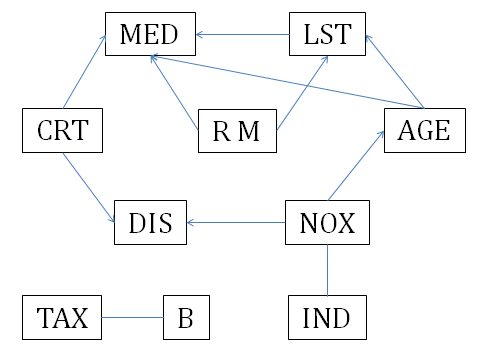
\includegraphics[width=0.55\linewidth]{img/res.png}
	\caption{The final result of PC algorithm, namely the causalities of the features in Boston Housing dataset.}
	\label{fig:pc-res}
\end{figure}

\vspace{-0.01\linewidth}
It is doubtless that this result meets the criterion perfectly. Besides, the $PC_{KCI-test}$ algorithm also finds out some other causalities that make sense (e.g. nitric oxides concentration (NOX) and distances to five Boston centres (DIS)).

\vspace{0.008\linewidth}
Nevertheless, I think $PC_{KCI-test}$ still omits some causalities that meet our common sense, such as DIS \footnote{The meaning of abbreviations can refer to \ref{apd:boston}} and TAX, IND and TAX, which could be discovered by $PC_{CI_{PERM}}$ algorithm according to the results in \cite{alg}. In the meantime, $PC_{KCI-test}$ also encounters difficulties in determining the causality between TAX and B, and ignores the causalities of two features (ZN and PTRATIO). 

\vspace{0.008\linewidth}
In conclusion, despite few blemishes described above, the KCI-test is a novel and efficient algorithm for independence testing, especially for \textbf{continuous variables} and \textbf{middle sample size}. The experiments on Boston Housing dataset indicates that $PC_{KCI-test}$ could achieve satisfactory results in both accuracy and speed under practical applications.

\vspace{-0.01\linewidth}
\section{Causal Tree Reconstruction}

Firstly, I consider three variables $x_1, x_2, x_3$, form their star decomposition, then choose a fourth variable $x_4$ and determine the leg where $x_4$ should be appended. Such leg could be found by testing which pairs of triplets share centers, deciding on appropriate topology, connecting $x_4$ accordingly.

\vspace{0.008\linewidth}
If there is a tree $T_i$, with $i$ leaves, ready to append the next, namely $(i + 1)th$, leaf. The solution is similar: choose any triplet of leaves from $T_i$ with central variable $w$, test which leg of $w$ the $x_{i+1}$ should append. This identifies a subtree $T_i^{'}$ of $T_i$ that should receive $x_{i+1}$ and permits me to remove from further consideration the subtrees emanating from the unselected legs of $w$.

\vspace{0.008\linewidth}
Repeating the above operations on the selected subtree $T_i^{'}$ would eventually reduce it to a single branch, to which $x_{i+1}$ is appended. The detailed construction procedure could be treated as two parts: 1) reconstructing rooted trees; 2) constructing unrooted tree.

\vspace{-0.02\linewidth}
\subsection{Reconstructing Root Trees}

Suppose $T$ is a rooted tree, with $n$ leaves $x_1, x_2, ... , x_n$, each node of $T$, which is not a leaf, has 2 to $k$ sons. $x_i$ is defined as the leader of the triple $(x_i, x_j, x_k)$ if the path from the root to it does not contain the deepest common ancestor of $x_j$ and $x_k$. Note that the deepest common ancestor of all the three leaves is also a common ancestor of any two of them if $(x_i, x_j, x_k)$ does not have a leader.

\vspace{0.008\linewidth}
The algorihm constructs a sequence of trees $T_2, T_3, ... , T_n$, where $T_2$ is a binary tree with three nodes and $T_n=T$. $T_{i+1}$ is constructed by appending $x_{i+1}$ as a new leaf to $T_i$. $T_i$ contains only the leaves $x_1, ... , x_i$ and corresponding edges, which would be the subtree of $T$. The location where $x_{i+1}$ should be appended to is determined by Alg. \ref{alg:append}. The lemmas used in the process can refer to Appendix \ref{apd:lemma}.

\vspace{0.01\linewidth}
\begin{algorithm}[H]
	\SetKwInOut{Input}{Input}
	\SetKwInOut{Output}{Output}
	\caption{Appending}
	\label{alg:append}
	\vspace{0.25\baselineskip}
	
	\Input{$T_i, x_{i+1}, i$}
	\Output{$T_{i+1}$}
	
	$T_c \leftarrow T_i$ ;
	
	$n \leftarrow $ the number of leaves in $T_c$ ;
	
	\If{$s = 2$}{
		$\overline{v} \leftarrow $ the root of $T_c$ ;
		$x_j, x_k \leftarrow$ the two leaves of $T_c$ ;
	}
	\ElseIf{$s > 2$}{
		$\overline{v} \leftarrow $ any node of $T_c$, for which
		\begin{equation*}
			\centering
			\dfrac{s}{k+1} < des(\overline{v} \leqslant \dfrac{sk}{k+1}) \quad (Lemma \; \ref{lemma:1}) ;
		\end{equation*}
		$x_j, x_k \leftarrow$ the two leaves whose common ancestor is $\overline{v}$ ;
	}
	
	Calculate the leader of $(x_{i+1}, x_j, x_k)$ (with respect to $T$) ;
	
	\If{$s = 2$}{
		\If{$x_j$ (or $x_k$) is the leader}{
			Append a new node on the edge of $x_k$ or $x_j$ respectively, making it the father of $x_{i+1}$ ;
		}
		\ElseIf{$x_{i+1}$ is the leader}{
			Append a new root, making $x_{i+1}$ and the old root $\overline{v}$ as its sons ;
		}
		\ElseIf{there is no leader}{
			Make $x_{i+1}$ as a son of $\overline{v}$ ;
		}
	}
	\ElseIf{$s > 2$}{
		Define a partition of $T_c$ into two subtrees: $T_{c1}$ rooted at $\overline{v}$ with all the descendants of $\overline{v}$ and $T_{c2} = T_c - T_{c1}$ in which $\overline{v}$ is considered as a leaf ;
		\If{$x_j$ (or $x_k$) is the leader}{
			$T_c \leftarrow $ the subtree of $T_{c1}$ rooted at that son of $\overline{v}$ which is the ancestor of $x_k$ (or $x_j$ respectively) ;
		}
		\ElseIf{$x_{i+1}$ is the leader of $x_{i+1}, x_j, x_k$}{
			$T_c \leftarrow T_{c2}$ ;
		}
		\ElseIf{there is no leader}{
			$T_c \leftarrow T_{c1}$, from which the two sons of $\overline{v}$ whose descendants are $x_j$ and $x_k$ are removed with all their descendants ;
		}
		
		Go to 2 ;
	}
	
	\Return $T_{i+1}$;
\end{algorithm}
\vspace{0.01\linewidth}

\subsection{Constructing Unrooted Trees}

Suppose $T$ is an unrooted tree in which the degree of each node is at least three, and suppose $u, v, w, x$ is any quadruple of leaves. Note that $x$ pairs with $u$ relative to $(v, w)$ if the path from $x$ to $u$ is edge-disjoint relative to the path from $v$ to $w$.

\vspace{0.008\linewidth}
Remove a leaf $x$ of $T$ and examine the remaining tree $T_1$ as rooted at the node $x_1$ with which $x$ is adjacent in $T$.

\vspace{0.008\linewidth}
Choosing arbitrarily a fixed leaf $x$, I can use Lemma \ref{lemma:2} and Alg. \ref{alg:append} to reconstruct $T_1$ rooted at $x_1$. Then appending $x$ as a son of $x_1$ to get the required tree $T$.

\newpage
\begin{appendix}
\section{Appendix}

\subsection{Details of the Boston Housing Dataset}
\label{apd:boston}

The Boston Housing Dataset consists of 506 samples, each has 12 features, namely the factors that affect housing price. The values of all features are positive real numbers. Table \ref{tab:boston} shows a detailed description of these features.

\begin{table}[H]
	\renewcommand\arraystretch{1.35}
	\caption{Details of the features in Boston Housing dataset}
	\label{tab:boston}
	\centering
	
	\begin{tabular}{c|c|c}
		\centering
		Identifier & Feature Names & Description \\
		\hline
		1 & CRIM & per capita crime rate by town \\
		2 & ZN & proportion of residential land zoned for lots over 25,000.000 sq.ft. \\
		3 & INDUS & proportion of non-retail business acres per town \\
		4 & NOX & nitric oxides concentration (parts per 10.0 million) \\
		5 & RM & average number of rooms per dwelling \\
		6 & AGE & proportion of owner-occupied units built prior to 1940.000 \\
		7 & DIS & weighted distances to five Boston employment centres \\
		8 & TAX & full-value property-tax rate per \$10,000.0 \\
		9 & PTRATIO & pupil-teacher ratio by town \\
		10 & B & 1000(Bk - 0.63)\^2 where Bk is the proportion of blacks by town \\
		11 & LSTAT & lower status of the population \\			
		12 & MEDV & Median value of owner-occupied homes in \$1000's \\
	\end{tabular}
\end{table}

\subsection{Lemmas}
\label{apd:lemma}

\begin{lemma}
	\label{lemma:1}
	Suppose k is the maximum number of sons of a node in a rooted tree T with n leaves. There exists a node v of T such that
	\begin{equation*}
		\centering
		\dfrac{n}{k+1} < des(v) \leqslant \dfrac{nk}{k+1},
	\end{equation*}
	where des(v) is defined to be the number of leaves which are descendants of v, and des(v) = 1 if v is a leaf.
\end{lemma}

\begin{lemma}
	\label{lemma:2}
	x pairs with u relative to (v, w) in the tree T if and only if u is the leader of u, v, w in the tree $T_1$ rooted at $x_1$.
\end{lemma}


\end{appendix}

\bibliographystyle{ieeetr}
\bibliography{bio}

\end{document}